\documentclass[conference]{IEEEtran}
\IEEEoverridecommandlockouts
\usepackage{cite}
\usepackage{amsmath,amssymb,amsfonts}
\usepackage{algorithmic}
\usepackage{graphicx}
\usepackage{textcomp}
\usepackage{xcolor}
\usepackage{booktabs}
\usepackage{float}
\usepackage{multirow}
\usepackage{siunitx}
\usepackage[hyphens]{url}

\def\BibTeX{{\rm B\kern-.05em{\sc i\kern-.025em b}\kern-.08em
    T\kern-.1667em\lower.7ex\hbox{E}\kern-.125emX}}

\graphicspath{{../results/plots/}}

\begin{document}

\title{Topological Risk Analysis and Criticality Mapping\\ in the npm Software Supply Chain}

\author{\IEEEauthorblockN{Yusuf Talha ARABACI}
\IEEEauthorblockA{\textit{Department of Software Engineering} \\
\textit{Karabuk University}\\
Karabuk, Turkey \\
yusuftalhaarabaci@hotmail.com}
}

\maketitle

\begin{abstract}
While centralized package managers like NPM accelerate software development by providing ready-to-use code libraries, the intricate web of nested dependencies among these components has transformed the ecosystem into a complex and fragile structure. Current security approaches remain insufficient in detecting these systemic risks, which stem from the network's structural architecture and possess the potential for cascading effects. This study aims to map systemic risks within the NPM ecosystem using topological analysis methods that are independent of package content. Within the scope of the analysis, a directed graph was constructed by modeling the top 1,000 packages with the most dependents in the NPM ecosystem, along with their dependencies extending up to a depth of 7. In-degree, out-degree, and betweenness metrics were calculated on the network, and a novel ``Behavioral Risk Score'' (BRS) was developed through a weighted combination of these values. The statistical distribution of the calculated metrics reveals that the network exhibits a scale-free topology; consequently, risk is concentrated on a small number of critical nodes that form the backbone of the ecosystem. Robustness simulations confirmed that the removal of packages with high BRS scores leads to a destructive collapse in network integrity. This research contributes a novel topology-based perspective to the literature by emphasizing that limited security resources should be directed toward the critical nodes forming the ecosystem's backbone, rather than relying on random scans.
\end{abstract}

\begin{IEEEkeywords}
Software supply chain security, npm, dependency network, topological analysis, risk scoring, network robustness.
\end{IEEEkeywords}

\section{Introduction}
Modern software engineering depends on centralized package managers such as npm, which host extensive repositories of reusable code libraries \cite{wyss2025npm}. While this modularity accelerates development, it creates a fragile software supply chain where single points of failure can propagate throughout the ecosystem \cite{duan2020measuring}. The npm ecosystem, characterized by millions of packages and complex inter-dependencies, presents a significant attack surface \cite{wang2023threat}. Vulnerabilities propagate through the dependency graph \cite{liu2022demystifying, zerouali2022impact}, and disruptions in package maintenance compound these systemic risks \cite{rahman2024update, cogo2020maintenance}.

Literature confirms that the npm network exhibits "small-world" characteristics, where a limited number of packages or maintainers exert disproportionate influence \cite{zimmermann2019smallworld, oldnall2017complex}. This topological structure exposes the ecosystem to supply chain attacks ranging from typosquatting to the compromise of trusted, popular packages \cite{ohm2020backstabber}. Although defense mechanisms utilizing machine learning, dynamic analysis, and metadata scanning have been proposed \cite{sejfia2022amalfi, zheng2024oscar, halder2024metadata}, the scale of the ecosystem renders comprehensive code-level scanning computationally prohibitive.

Existing research typically quantifies risk based on known vulnerabilities or maintenance status. However, few approaches quantify systemic risk derived solely from the network's topological architecture. This study addresses this gap by introducing a content-independent model that focuses exclusively on structural dependencies. We propose the \textbf{Behavioral Risk Score (BRS)}, a composite metric weighting various centrality measures to prioritize structurally critical packages. The objective is to provide a quantitative framework for security resource allocation, facilitating strategic defense against systemic supply chain threats.

\section{Methodology}
\subsection{Dataset and Network Construction}
We adopted a \textbf{Combined Sampling Strategy} to ensure the network model captures both infrastructural backbone packages and widely consumed end-user tools. We selected the top 1,000 packages by \textbf{dependents count} (infrastructure) and the top 1,000 packages by \textbf{download count} (popularity) from the \texttt{ecosyste.ms} dataset. Merging these lists resulted in a unique seed set of 1,452 packages. All dependencies of this seed set were traversed up to a depth of seven. Following preprocessing to remove circular references, we constructed a directed graph of \textbf{1,506 nodes (packages)} and \textbf{3,058 edges (dependencies)}. The Python NetworkX library was employed for network modeling and analysis.

\subsection{The Behavioral Risk Score (BRS) Model}
The BRS is a composite score designed to quantify a package's structural risk. It synthesizes multiple metrics to integrate the network's topological structure with the package's ecosystem prevalence.

We calculated the following centrality metrics for each package:
\begin{itemize}
    \item \textbf{In-Degree:} The count of incoming dependencies, indicating popularity and direct impact radius \cite{freeman1978centrality}.
    \item \textbf{Out-Degree:} The count of outgoing dependencies. High out-degree suggests an expanded attack surface \cite{newman2010networks}.
    \item \textbf{Betweenness Centrality:} The frequency with which a node appears on shortest paths between other nodes, quantifying its role as a network "bridge" \cite{freeman1978centrality}.
    \item \textbf{Inverted Clustering Coefficient:} A measure of local network fragility. We interpret low clustering (structural holes) as high risk, calculated as $1 - \text{ClusteringCoefficient}$ \cite{watts1998smallworld}.
\end{itemize}
In addition to topological metrics, \textbf{Dependents Count} and \textbf{Download Count} were included as proxies for global adoption.

Metrics were normalized to the $[0,1]$ range using Min-Max scaling. To address heavy-tailed distributions, \textbf{Dependents Count}, \textbf{Download Count}, and \textbf{Staleness} were log-normalized prior to scaling:
\begin{equation}
x' = \frac{\ln(1+x) - \min(\ln(1+x))}{\max(\ln(1+x)) - \min(\ln(1+x))}
\end{equation}

The final BRS is computed as a weighted sum:
$$
\begin{aligned}
\text{BRS} = & \ 0.35 \cdot \text{Betweenness}' + 0.30 \cdot \text{InDegree}' \\
& + 0.15 \cdot \text{ClusteringInv}' + 0.10 \cdot \text{OutDegree}' \\
& + 0.05 \cdot \text{Dependents}' + 0.05 \cdot \text{Downloads}'
\end{aligned}
$$

The weighting rationale is as follows:
\begin{itemize}
    \item \textbf{Betweenness ($w=0.35$)}: Assigned the highest weight to prioritize "bridge" nodes controlling information and risk flow.
    \item \textbf{In-Degree ($w=0.30$)}: Represents direct impact radius and immediate reach.
    \item \textbf{Inverted Clustering ($w=0.15$)}: Captures local fragility; nodes bridging distinct clusters without redundant connections pose higher systemic risk.
    \item \textbf{Out-Degree ($w=0.10$)}: Accounts for the expanded attack surface from upstream dependencies.
    \item \textbf{Global Metrics ($w=0.05$ each)}: Dependents and Downloads are given lower weightings to prioritize structural topology over raw popularity.
\end{itemize}

\subsection{Robustness and Cascade Analysis}
To validate the model, we performed targeted attack simulations. We analyzed the impact of removing high-BRS packages on the Largest Connected Component (LCC) size and overall network accessibility. A cascade analysis further verified the predictive power of the model.

\section{Results and Discussion}

\subsection{Network Topology and Structural Characteristics}
The dependency network demonstrates a clustered topology (Figure \ref{fig:network}) and a scale-free structure. Degree distributions for both in-degree and out-degree exhibit heavy tails (Figure \ref{fig:histograms}), consistent with scale-free networks. This implies that a minority of packages function as central hubs, while the majority possess few connections. Consequently, systemic risk is not uniformly distributed but concentrated within a subset of critical packages.

\begin{figure}[H]
\centering
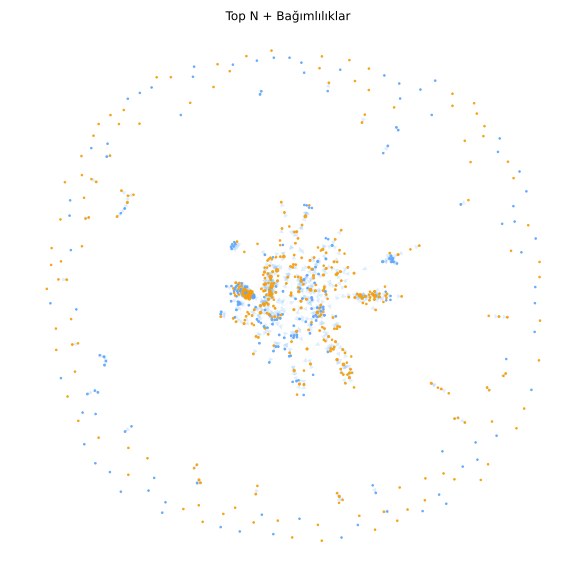
\includegraphics[width=\linewidth]{network_full_topN.png}
\caption{Visualization of the dependency network. Dense regions indicate distinct sub-clusters.}
\label{fig:network}
\end{figure}

\begin{figure}[H]
\centering
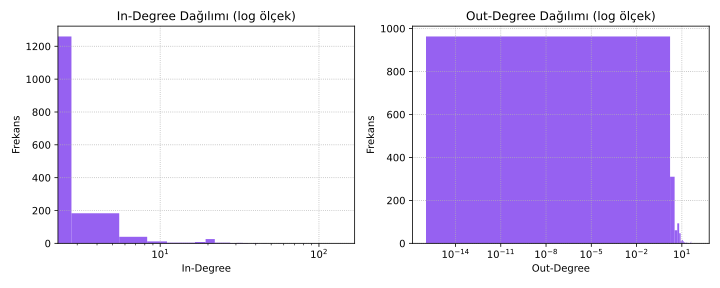
\includegraphics[width=\linewidth]{degree_histograms.png}
\caption{In-degree and out-degree histograms, showing heavy-tailed distributions characteristic of scale-free networks.}
\label{fig:histograms}
\end{figure}

\subsection{Centrality Relationships}
Analysis of centrality measures indicates an asymmetric relationship between popularity (in-degree) and structural importance (betweenness centrality), as illustrated in Figure \ref{fig:scatter}. The weak correlation suggests that packages with low popularity may effectively sustain network integrity by connecting disparate components. Security analyses focusing exclusively on popularity metrics, such as download counts, are therefore likely to overlook these structural risks.

\begin{figure}[H]
\centering
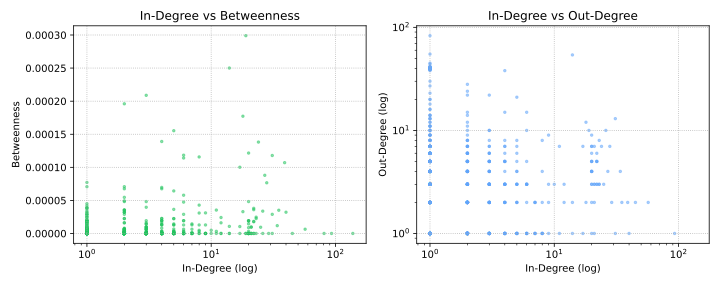
\includegraphics[width=\linewidth]{scatter_correlations.png}
\caption{Correlations between network centrality measures.}
\label{fig:scatter}
\end{figure}

\subsection{Analysis of Critical Nodes}
Tables \ref{tab:indegree}, \ref{tab:outdegree}, and \ref{tab:betweenness} enumerate the top 10 packages for each centrality measure. High in-degree packages, such as \texttt{@babel/helper-plugin-utils}, are widely utilized dependencies. High out-degree packages, like \texttt{@babel/preset-env}, exhibit numerous dependencies, indicating a broader attack surface. High betweenness centrality packages are critical for network integrity, acting as bridges. For instance, \texttt{jest-circus} possesses a low in-degree of 1 but the highest betweenness score, underscoring its role as a structural bridge. conversely, \texttt{@babel/core} exhibits both high popularity and high betweenness. These results demonstrate that single metrics are insufficient for comprehensive risk analysis, necessitating the identification of structurally critical bridge packages.

\begin{table}[H]
\centering
\caption{\textsc{Top 10 Packages by In-Degree Centrality}}
\label{tab:indegree}
\resizebox{\linewidth}{!}{%
\begin{tabular}{lrrrr}
\toprule
Package & In-Degree & Out-Degree & Betweenness & TopN? \\
\midrule
tslib & 156 & 0 & 0.000000 & True \\
@babel/helper-plugin-utils & 110 & 0 & 0.000000 & True \\
@smithy/types & 94 & 1 & 0.000000 & True \\
@aws-sdk/types & 57 & 2 & 0.000001 & True \\
debug & 51 & 1 & 0.000035 & True \\
@smithy/protocol-http & 45 & 2 & 0.000000 & True \\
@types/node & 42 & 1 & 0.000015 & True \\
call-bound & 41 & 2 & 0.000036 & True \\
postcss-value-parser & 39 & 0 & 0.000000 & True \\
call-bind & 36 & 4 & 0.000055 & True \\
\bottomrule
\end{tabular}%
}
\end{table}

\begin{table}[H]
\centering
\caption{\textsc{Top 10 Packages by Out-Degree Centrality}}
\label{tab:outdegree}
\resizebox{\linewidth}{!}{%
\begin{tabular}{lrrrr}
\toprule
Package & Out-Degree & In-Degree & Betweenness & TopN? \\
\midrule
telecom-mas-agent & 83 & 1 & 0.000000 & True \\
@babel/preset-env & 70 & 3 & 0.000084 & True \\
postcss-preset-env & 69 & 1 & 0.000000 & True \\
@aws-sdk/client-s3 & 55 & 1 & 0.000009 & False \\
es-abstract & 54 & 17 & 0.000319 & True \\
react-scripts & 48 & 0 & 0.000000 & True \\
@aws-sdk/client-s3-control & 45 & 1 & 0.000002 & False \\
@aws-sdk/client-lambda & 44 & 1 & 0.000003 & False \\
cypress & 42 & 1 & 0.000037 & False \\
@aws-sdk/client-dynamodb & 42 & 1 & 0.000004 & False \\
\bottomrule
\end{tabular}%
}
\end{table}

\begin{table}[H]
\centering
\caption{\textsc{Top 10 Packages by Betweenness Centrality}}
\label{tab:betweenness}
\resizebox{\linewidth}{!}{%
\begin{tabular}{lrrrr}
\toprule
Package & Betweenness & In-Degree & Out-Degree & TopN? \\
\midrule
es-abstract & 0.000319 & 17 & 54 & True \\
jest-snapshot & 0.000183 & 6 & 21 & True \\
@babel/core & 0.000151 & 12 & 15 & True \\
@babel/traverse & 0.000150 & 20 & 7 & True \\
workbox-build & 0.000143 & 1 & 37 & True \\
@jest/transform & 0.000115 & 6 & 15 & True \\
get-intrinsic & 0.000111 & 22 & 10 & True \\
jest & 0.000086 & 2 & 4 & True \\
@babel/preset-env & 0.000084 & 3 & 70 & True \\
browserslist & 0.000083 & 16 & 5 & True \\
\bottomrule
\end{tabular}%
}
\end{table}

\subsection{Composite Risk Score (BRS) Ranking}
The BRS model synthesizes popularity, attack surface, and strategic position into a unified metric. As depicted in Figure \ref{fig:risk_scores} and Table \ref{tab:risk}, packages rank highly on the BRS scale due to aggregate scores across dimensions. This ranking provides a prioritized list for security audit resource allocation.

\begin{figure}[H]
\centering
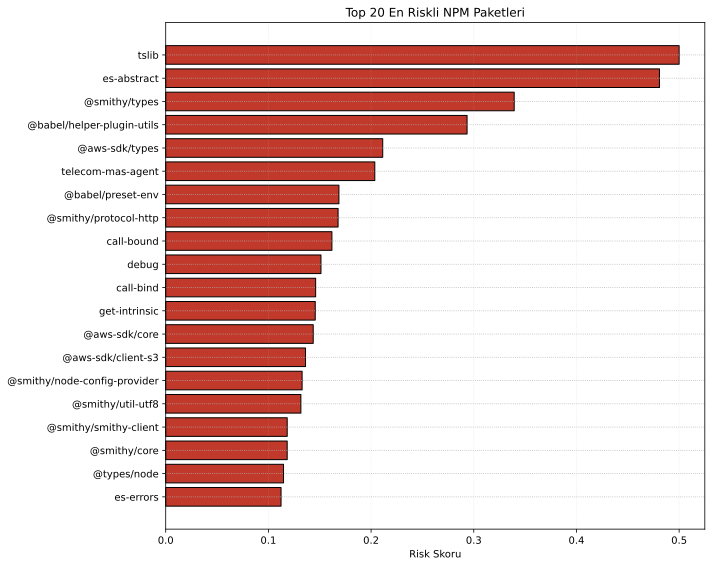
\includegraphics[width=\linewidth]{top20_risk_scores.png}
\caption{Top 20 packages by Composite Risk Score (BRS).}
\label{fig:risk_scores}
\end{figure}

\begin{table}[H]
\centering
\caption{\textsc{Top 20 Packages by Composite Risk Score (BRS)}}
\label{tab:risk}
\resizebox{\linewidth}{!}{%
\begin{tabular}{lrrrrr}
\toprule
Package & Risk & In-Degree & Out-Degree & Betweenness & TopN? \\
\midrule
es-abstract & 0.663705 & 17 & 54 & 0.000319 & True \\
tslib & 0.536811 & 156 & 0 & 0.000000 & True \\
jest-snapshot & 0.462890 & 6 & 21 & 0.000183 & True \\
@babel/helper-plugin-utils & 0.452984 & 110 & 0 & 0.000000 & True \\
@babel/traverse & 0.448099 & 20 & 7 & 0.000150 & True \\
@babel/core & 0.442809 & 12 & 15 & 0.000151 & True \\
workbox-build & 0.431952 & 1 & 37 & 0.000143 & True \\
@babel/preset-env & 0.419845 & 3 & 70 & 0.000084 & True \\
get-intrinsic & 0.404645 & 22 & 10 & 0.000111 & True \\
@smithy/types & 0.392332 & 94 & 1 & 0.000000 & True \\
debug & 0.380693 & 51 & 1 & 0.000035 & True \\
@jest/transform & 0.377578 & 6 & 15 & 0.000115 & True \\
call-bind & 0.366630 & 36 & 4 & 0.000055 & True \\
browserslist & 0.366479 & 16 & 5 & 0.000083 & True \\
@jest/types & 0.362285 & 26 & 7 & 0.000072 & True \\
@babel/types & 0.348737 & 32 & 2 & 0.000041 & True \\
@types/node & 0.332670 & 42 & 1 & 0.000015 & True \\
@babel/helper-compilation-targets & 0.331183 & 7 & 5 & 0.000073 & True \\
@jest/core & 0.330805 & 2 & 28 & 0.000069 & True \\
@aws-sdk/credential-provider-node & 0.327093 & 18 & 12 & 0.000061 & True \\
\bottomrule
\end{tabular}%
}
\end{table}

\subsection{Systemic Impact and Cascade Analysis}
Simulation results corroborate the validity of the BRS model. Figure \ref{fig:impact} illustrates that the removal of high-BRS packages precipitates a significant reduction in LCC size. The correlation between the BRS score and the resulting cascade effect (Figure \ref{fig:cascade}) affirms the metric's utility for risk prediction.

\begin{figure}[H]
\centering
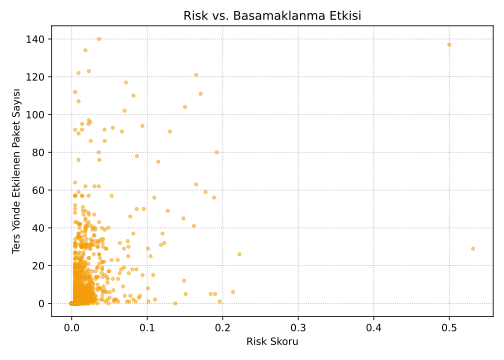
\includegraphics[width=\linewidth]{risk_vs_cascade.png}
\caption{Relationship between BRS and cascade effect, measured by network accessibility.}
\label{fig:cascade}
\end{figure}

\begin{figure}[H]
\centering
\includegraphics[width=\linewidth]{top20_cascade_impact.png}
\caption{Effect of removing the top 20 high-BRS packages on LCC size and network accessibility.}
\label{fig:impact}
\end{figure}

\section{Discussion}
This study presented the Composite Risk Score (BRS), a model quantifying structural risks in the npm ecosystem, advancing beyond descriptive analyses. The BRS ranking facilitates the operational prioritization of security resources. Our analysis demonstrates that network resilience relies not only on popular packages but also on infrastructural "bridge" packages such as \texttt{jest-circus} and \texttt{@babel/core}. These findings align with the "small-world" network structure identified by Zimmermann et al. \cite{zimmermann2019smallworld}, while extending the literature by highlighting risk concentration in intermediate-layer bridge packages.

"Cascade Impact" simulations were performed on the constructed dependency graph as a proxy for the entire npm registry due to computational constraints. This methodology relies on the "supply chain backbone" hypothesis, where the topological disintegration of this dense network of critical packages serves as a proxy for functional failure in dependent projects. The structural collapse of this local backbone acts as an indicator of global systemic risk.

\section{Limitations}
This analysis is confined to static dependencies defined in \texttt{package.json} files, excluding dynamic runtime loading and developer account reputation. The analysis represents a static snapshot and does not capture temporal evolution. Legal risks, such as license compliance, remain outside the scope of this study \cite{ahlstrom2025licensing}.

\section{Conclusion}
This study proposed a topology-based methodology for identifying and prioritizing structurally critical packages in the npm software supply chain. By synthesizing multiple network metrics into the Behavioral Risk Score (BRS), we provided a quantitative framework to guide security resource allocation. Findings indicate that prioritizing structurally critical nodes offers a more efficient strategy for mitigating systemic risk than focusing on popularity alone. Future research should expand the model to incorporate developer social networks and maintenance behaviors, and apply the methodology to other package ecosystems to derive generalized supply chain security models.

\section{Reproducibility}
Source code and datasets are available to ensure reproducibility:
\begin{itemize}
  \item \textbf{Analysis Code:} Hosted in \texttt{analysis/analysis.ipynb} (Python 3, NetworkX, pandas).
  \item \textbf{Data Outputs:} Intermediate results and metrics are available in CSV format in the \texttt{results/} directory.
\end{itemize}

% APA-style bibliography 
\begin{thebibliography}{30}

\bibitem{lit1} E. Wyss, ``A new frontier for software security: Diving deep into npm,'' 2025.

\bibitem{lit7} M. Wang, P. Wu, and Q. Luo, ``Construction of software supply chain threat portrait based on chain perspective,'' 2023.

\bibitem{lit8} C. Liu et al., ``Demystifying vulnerability propagation via dependency trees in npm,'' in \textit{ICSE}, 2022.

\bibitem{lit18} A. Zerouali et al., ``On the impact of security vulnerabilities in the npm and RubyGems dependency networks,'' 2022.

\bibitem{lit5} I. Rahman et al., ``Characterizing dependency update practice of NPM, PyPI and Cargo packages,'' 2024.

\bibitem{lit22} F. R. Cogo, ``Studying dependency maintenance practices through mining NPM,'' 2020.

\bibitem{lit10} A. J. Jafari et al., ``Dependency practices for vulnerability mitigation,'' 2023.

\bibitem{lit20} M. Zimmermann et al., ``Small world with high risks: Security threats in npm,'' in \textit{USENIX Sec.}, 2019.

\bibitem{lit16} A. Hafner, A. Mur, and J. Bernard, ``Node package manager's dependency network robustness,'' 2021.

\bibitem{lit25} E.-R. Oldnall, ``The web of dependencies: A complex network analysis of the NPM,'' 2017.

\bibitem{lit2} P. Jaisri, B. Reid, and R. G. Kula, ``A preliminary study on self-contained libraries in the NPM ecosystem,'' 2024.

\bibitem{lit6} T. G. Hastings, ``Combating source poisoning and next-generation software supply chain attacks,'' 2024.

\bibitem{lit30} M. Shcherbakov, P. Moosbrugger, and M. Balliu, ``Unveiling the invisible: Prototype pollution gadgets via dynamic taint,'' 2021.

\bibitem{lit12} D. Y. K. Yip, ``Empirical study on dependency-based attacks in Node.js,'' 2022.

\bibitem{lit4} M. Ohm et al., ``Backstabber's knife collection: A review of open source software supply chain attacks,'' in \textit{DIMVA}, 2020.

\bibitem{lit24} P. Ladisa et al., ``The hitchhiker's guide to malicious third-party dependencies,'' in \textit{IEEE S\&P}, 2023.

\bibitem{lit28} R. Duan et al., ``Towards measuring supply chain attacks on package managers,'' in \textit{NDSS}, 2020.

\bibitem{lit19} A. Sejfia and M. Schafer, ``Practical automated detection of malicious npm packages (Amalfi),'' in \textit{ICSE}, 2022.

\bibitem{lit29} X. Zheng et al., ``Towards robust detection of OSS supply chain poisoning (OSCAR),'' 2024.

\bibitem{lit15} S. Halder et al., ``Malicious package detection using metadata information,'' 2024.

\bibitem{lit14} J. Zhang et al., ``Malicious package detection in NPM and PyPI using a single model of malicious behavior sequence,'' 2023.

\bibitem{lit17} P. Ladisa et al., ``On the feasibility of cross-language detection of malicious packages in npm and PyPI,'' 2023.

\bibitem{lit11} M. L. P. Correia, ``Detection of software supply chain attacks in code repositories,'' 2022.

\bibitem{lit23} M. Ohm et al., ``Supporting detection via unsupervised signature generation (ACME),'' 2021.

\bibitem{lit13} S. Torres-Arias, ``In-toto: Practical software supply chain security,'' in \textit{USENIX Sec.}, 2020.

\bibitem{lit3} S. Yu, ``Accurate and efficient SBOM generation for software supply chain security,'' 2024.

\bibitem{lit9} H. E. Ahlstrom, ``Dependency analysis for software licensing and security,'' 2025.

\bibitem{lit21} T. R. Schorlemmer, ``Software supply chain security: Attacks, defenses, and signing adoption,'' 2024.

\bibitem{lit26} N. Imtiaz, ``Toward secure use of open source dependencies,'' 2023.

\bibitem{lit27} S. Vaidya, ``Towards ensuring integrity and authenticity of software repositories,'' 2022.

\end{thebibliography}


\end{document}
